\documentclass[tikz,border=4pt]{standalone}
\usepackage[scaled=0.92]{helvet}
\renewcommand{\familydefault}{\sfdefault}
\usepackage{amsmath,amssymb}
\usetikzlibrary{positioning,arrows.meta,calc,fit,backgrounds,shapes.geometric,decorations.pathreplacing}

% ---- palette ----
\definecolor{ink}{HTML}{1F2328}
\definecolor{muted}{HTML}{6B6A66}
\definecolor{line}{HTML}{C9C7C0}
\definecolor{paper}{HTML}{F7F6F2}
\definecolor{blue}{HTML}{2A78D6}
\definecolor{blueL}{HTML}{E4EEFA}
\definecolor{orange}{HTML}{EB6834}
\definecolor{orangeL}{HTML}{FCE9E1}
\definecolor{aqua}{HTML}{1BAF7A}
\definecolor{aquaL}{HTML}{E0F4EC}
\definecolor{violet}{HTML}{6250D6}
\definecolor{violetL}{HTML}{ECE9FA}
\definecolor{amber}{HTML}{C98500}
\definecolor{amberL}{HTML}{FBF1DC}

\tikzset{
  >={Stealth[length=5pt,width=4pt]},
  panel/.style={draw=line, line width=0.6pt, rounded corners=6pt, fill=paper},
  card/.style={draw=line, line width=0.5pt, rounded corners=4pt, fill=white},
  stage/.style={draw=#1, line width=0.7pt, rounded corners=4pt, fill=#1!8, minimum height=9mm, align=center, font=\scriptsize\color{ink}},
  chip/.style={rounded corners=2pt, fill=#1, text=white, font=\tiny\bfseries, inner sep=2pt, minimum height=3.6mm},
  stepn/.style={circle, fill=ink, text=white, font=\tiny\bfseries, inner sep=0.6pt, minimum size=3.6mm},
  flow/.style={->, line width=0.8pt, color=ink},
  soft/.style={->, line width=0.6pt, color=muted, dashed},
  title/.style={font=\footnotesize\bfseries\color{ink}, anchor=north west},
  sub/.style={font=\tiny\color{muted}, anchor=north west},
}

% mini label histogram for a non-IID client
\newcommand{\hist}[6]{% x y h1 h2 h3 h4 (heights mm)
  \foreach \h [count=\i] in {#3,#4,#5,#6}{
    \pgfmathsetmacro{\xx}{#1+(\i-1)*0.17}
    \ifcase\i\or\def\cc{blue}\or\def\cc{orange}\or\def\cc{aqua}\or\def\cc{violet}\fi
    \fill[\cc, rounded corners=0.4pt] (\xx,#2) rectangle ++(0.12,\h/10);
  }
  \draw[line, line width=0.4pt] (#1-0.04,#2) -- (#1+0.68,#2);
}

\begin{document}
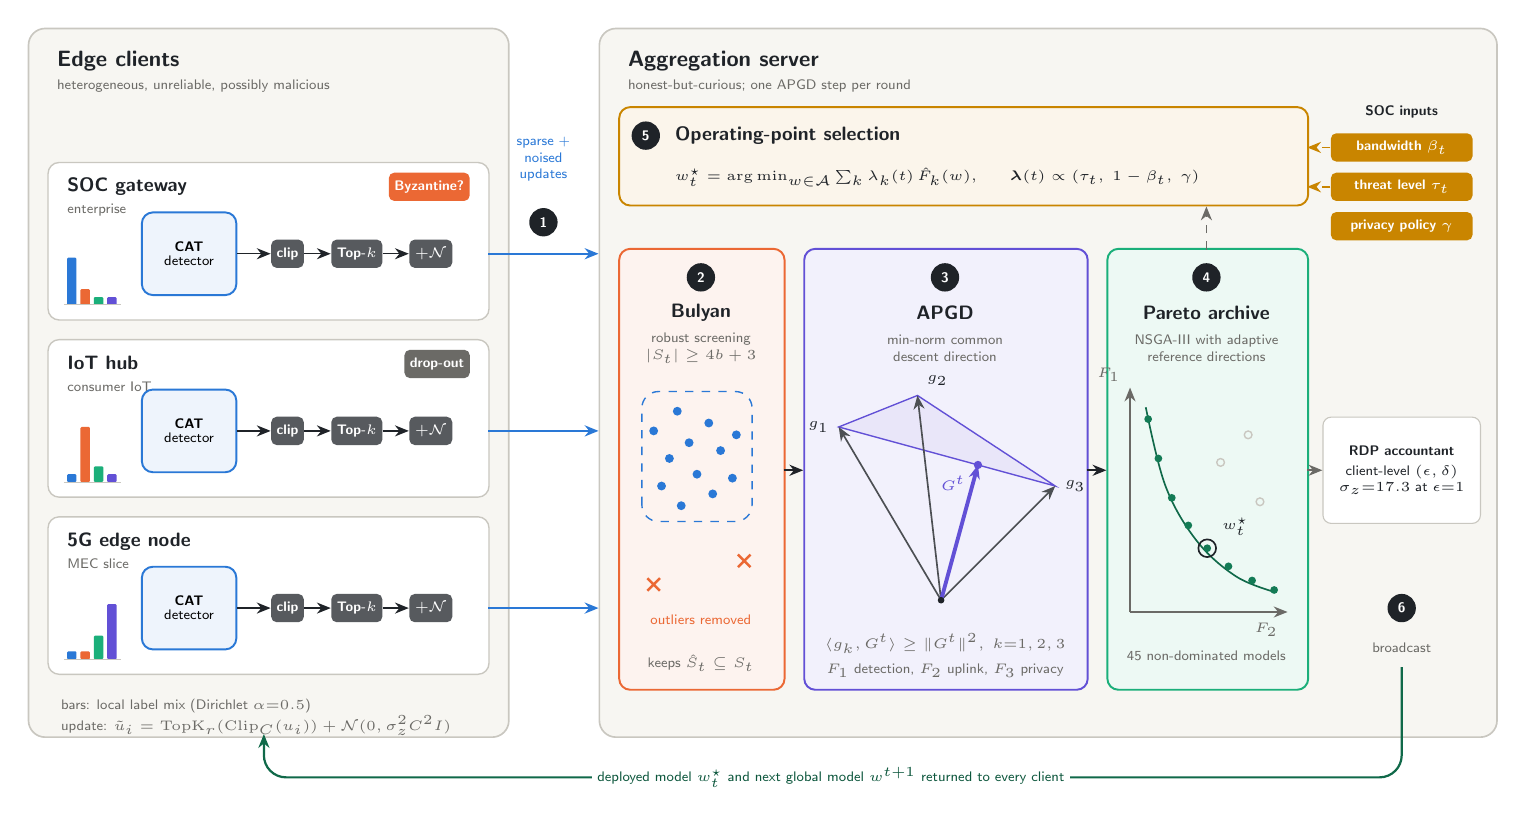
\begin{tikzpicture}[x=1cm,y=1cm]

% =================== CLIENT PANEL ===================
\node[panel, minimum width=6.1cm, minimum height=9.0cm, anchor=south west] (P1) at (0,0) {};
\node[title] at (0.25,8.85) {Edge clients};
\node[sub] at (0.25,8.48) {heterogeneous, unreliable, possibly malicious};

\foreach \yy/\nm/\sb/\a/\b/\c/\d/\tag in {
    6.2/SOC gateway/enterprise/6/2/1/1/c1,
    3.95/IoT hub/consumer IoT/1/7/2/1/c2,
    1.7/5G edge node/MEC slice/1/1/3/7/c3}{
  \node[card, minimum width=5.6cm, minimum height=2.0cm, anchor=south west] (\tag) at (0.25,\yy-0.9) {};
  \node[font=\scriptsize\bfseries\color{ink}, anchor=north west] at (0.38,\yy+1.03) {\nm};
  \node[font=\tiny\color{muted}, anchor=north west] at (0.38,\yy+0.7) {\sb};
  \hist{0.5}{\yy-0.7}{\a}{\b}{\c}{\d}
  \node[stage=blue, minimum width=1.2cm, minimum height=1.05cm, font=\tiny] (cat\tag) at (2.05,\yy-0.05) {\textbf{CAT}\\[-1pt]detector};
  \node[chip=ink!75] (k1\tag) at (3.3,\yy-0.05) {clip};
  \node[chip=ink!75] (k2\tag) at (4.18,\yy-0.05) {Top-$k$};
  \node[chip=ink!75] (k3\tag) at (5.12,\yy-0.05) {$+\mathcal{N}$};
  \draw[->, line width=0.5pt, color=ink] (cat\tag.east) -- (k1\tag.west);
  \draw[->, line width=0.5pt, color=ink] (k1\tag) -- (k2\tag);
  \draw[->, line width=0.5pt, color=ink] (k2\tag) -- (k3\tag);
}
\node[chip=orange] at (5.1,7.0) {Byzantine?};
\node[chip=muted] at (5.2,4.75) {drop-out};
\node[font=\tiny\color{muted}, anchor=north west, align=left] at (0.3,0.62) {bars: local label mix (Dirichlet $\alpha{=}0.5$)\\update: $\tilde u_i=\mathrm{TopK}_r(\mathrm{Clip}_C(u_i))+\mathcal{N}(0,\sigma_z^2C^2I)$};

% =================== UPLINK ===================
\foreach \yy in {6.15, 3.9, 1.65}{
  \draw[flow, color=blue] (5.85,\yy) -- (7.25,\yy);
}
\node[stepn] at (6.55,6.55) {1};
\node[font=\tiny\color{blue}, align=center] at (6.55,7.35) {sparse +\\noised\\updates};

% =================== SERVER PANEL ===================
\node[panel, minimum width=11.4cm, minimum height=9.0cm, anchor=south west] (P2) at (7.25,0) {};
\node[title] at (7.5,8.85) {Aggregation server};
\node[sub] at (7.5,8.48) {honest-but-curious; one APGD step per round};

% Bulyan
\node[stage=orange, minimum width=2.1cm, minimum height=5.6cm, anchor=south west] (bul) at (7.5,0.6) {};
\node[stepn] at (8.55,5.85) {2};
\node[font=\scriptsize\bfseries\color{ink}] at (8.55,5.4) {Bulyan};
\node[font=\tiny\color{muted}, align=center] at (8.55,4.95) {robust screening\\$|S_t|\ge 4b+3$};
\foreach \x/\y in {7.95/3.9, 8.25/4.15, 8.4/3.75, 8.15/3.55, 8.65/4.0, 8.8/3.65, 8.5/3.35, 9.0/3.85, 8.05/3.2, 8.7/3.1, 8.3/2.95, 8.95/3.3}{
  \fill[blue] (\x,\y) circle (1.6pt);
}
\draw[blue, line width=0.5pt, dashed, rounded corners=6pt] (7.8,2.75) rectangle (9.2,4.4);
\foreach \x/\y in {7.95/1.95, 9.1/2.25}{
  \draw[orange, line width=0.9pt] (\x-0.08,\y-0.08) -- (\x+0.08,\y+0.08) (\x-0.08,\y+0.08) -- (\x+0.08,\y-0.08);
}
\node[font=\tiny\color{orange}] at (8.55,1.5) {outliers removed};
\node[font=\tiny\color{muted}] at (8.55,0.95) {keeps $\hat S_t\subseteq S_t$};

% APGD
\node[stage=violet, minimum width=3.6cm, minimum height=5.6cm, anchor=south west] (apgd) at (9.85,0.6) {};
\node[stepn] at (11.65,5.85) {3};
\node[font=\scriptsize\bfseries\color{ink}] at (11.65,5.4) {APGD};
\node[font=\tiny\color{muted}, align=center] at (11.65,4.95) {min-norm common\\descent direction};
\coordinate (O) at (11.6,1.75);
\coordinate (G1) at (10.3,3.95);
\coordinate (G2) at (11.3,4.35);
\coordinate (G3) at (13.05,3.2);
\fill[violet!14] (G1) -- (G2) -- (G3) -- cycle;
\draw[violet, line width=0.5pt] (G1) -- (G2) -- (G3) -- cycle;
\foreach \p/\t/\pos in {G1/{g_1}/left, G2/{g_2}/above right, G3/{g_3}/right}{
  \draw[->, line width=0.6pt, color=ink!80] (O) -- (\p);
  \node[font=\tiny\color{ink}, \pos=0pt] at (\p) {$\t$};
}
% projection of O onto segment G1-G3
\path let \p1=($(G3)-(G1)$), \p2=($(O)-(G1)$) in
  \pgfextra{\pgfmathsetmacro{\tt}{(\x1*\x2+\y1*\y2)/(\x1*\x1+\y1*\y1)}\xdef\tproj{\tt}};
\coordinate (G) at ($(G1)!\tproj!(G3)$);
\draw[->, line width=1.4pt, color=violet] (O) -- (G);
\fill[violet] (G) circle (1.5pt);
\node[font=\tiny\bfseries\color{violet}, anchor=north east] at ($(G)+(-0.04,-0.02)$) {$G^t$};
\fill[ink] (O) circle (1.2pt);
\node[font=\tiny\color{muted}, align=center] at (11.65,1.2) {$\langle g_k,G^t\rangle\ge\|G^t\|^2,\ k{=}1,2,3$};
\node[font=\tiny\color{muted}, align=center] at (11.65,0.85) {$F_1$ detection, $F_2$ uplink, $F_3$ privacy};

% Archive
\node[stage=aqua, minimum width=2.55cm, minimum height=5.6cm, anchor=south west] (arc) at (13.7,0.6) {};
\node[stepn] at (14.97,5.85) {4};
\node[font=\scriptsize\bfseries\color{ink}] at (14.97,5.4) {Pareto archive};
\node[font=\tiny\color{muted}, align=center] at (14.97,4.95) {NSGA-III with adaptive\\reference directions};
\draw[->, line width=0.5pt, color=muted] (14.0,1.6) -- (16.0,1.6);
\node[font=\tiny, color=muted, anchor=north east] at (16.0,1.58) {$F_2$};
\draw[->, line width=0.5pt, color=muted] (14.0,1.6) -- (14.0,4.45);
\node[font=\tiny, color=muted, anchor=south east] at (14.0,4.4) {$F_1$};
\draw[aqua!60!black, line width=0.6pt] plot[smooth, tension=0.6] coordinates {(14.2,4.2) (14.45,3.2) (14.85,2.5) (15.35,2.05) (15.85,1.85)};
\foreach \p in {(14.23,4.05),(14.36,3.55),(14.53,3.05),(14.74,2.7),(14.98,2.41),(15.25,2.18),(15.55,2.0),(15.83,1.88)}{
  \fill[aqua!70!black] \p circle (1.4pt);
}
\draw[ink, line width=0.6pt] (14.98,2.41) circle (3.2pt);
\node[font=\tiny\color{ink}, anchor=south west] at (15.05,2.45) {$w^\star_t$};
\foreach \p in {(15.15,3.5),(15.65,3.0),(15.5,3.85)}{\draw[line, line width=0.5pt] \p circle (1.4pt);}
\node[font=\tiny\color{muted}] at (14.97,1.05) {45 non-dominated models};

\draw[flow] (9.6,3.4) -- (9.85,3.4);
\draw[flow] (13.45,3.4) -- (13.7,3.4);

% Selector strip
\node[stage=amber, minimum width=8.75cm, minimum height=1.25cm, anchor=south west] (sel) at (7.5,6.75) {};
\node[stepn] at (7.85,7.65) {5};
\node[font=\scriptsize\bfseries\color{ink}, anchor=west] at (8.1,7.65) {Operating-point selection};
\node[font=\tiny\color{ink}, anchor=west] at (8.1,7.12) {$w^\star_t=\arg\min_{w\in\mathcal{A}}\sum_k\lambda_k(t)\,\hat F_k(w),\qquad \boldsymbol\lambda(t)\propto(\tau_t,\ 1-\beta_t,\ \gamma)$};
\draw[soft] (14.97,6.2) -- (14.97,6.75);

% right column: inputs + accountant
\node[font=\tiny\bfseries\color{ink}] at (17.45,7.95) {SOC inputs};
\node[chip=amber, minimum width=1.8cm] (bw) at (17.45,7.5) {bandwidth $\beta_t$};
\node[chip=amber, minimum width=1.8cm] (th) at (17.45,7.0) {threat level $\tau_t$};
\node[chip=amber, minimum width=1.8cm] (pr) at (17.45,6.5) {privacy policy $\gamma$};
\draw[soft, color=amber] (bw.west) -- (16.25,7.5);
\draw[soft, color=amber] (th.west) -- (16.25,7.0);
\node[draw=line, rounded corners=3pt, fill=white, minimum width=2.0cm, minimum height=1.35cm, align=center, font=\tiny\color{ink}] (rdp) at (17.45,3.4) {\textbf{RDP accountant}\\[1pt]client-level $(\epsilon,\delta)$\\$\sigma_z{=}17.3$ at $\epsilon{=}1$};
\draw[soft] (16.25,3.4) -- (rdp.west);
\node[stepn] at (17.45,1.65) {6};
\node[font=\tiny\color{muted}, align=center] at (17.45,1.15) {broadcast};

% =================== DOWNLINK ===================
\draw[flow, color=aqua!60!black, rounded corners=8pt] (17.45,0.9) -- (17.45,-0.5) -- (3.0,-0.5) -- (3.0,0.05);
\node[font=\tiny\color{aqua!50!black}, fill=white, inner sep=2pt] at (10.2,-0.5) {deployed model $w^\star_t$ and next global model $w^{t+1}$ returned to every client};

\end{tikzpicture}
\end{document}
